\documentclass[a4paper]{IEEEtran}
\IEEEoverridecommandlockouts
% The preceding line is only needed to identify funding in the first footnote. If that is unneeded, please comment it out.
\usepackage{}
\usepackage{amsmath,amssymb,amsfonts}
\usepackage{algorithmic}
\usepackage{graphicx}
\usepackage{textcomp}
\usepackage{xcolor}
\usepackage[font=normalsize,labelfont=bf]{caption}


\def\BibTeX{{\rm B\kern-.05em{\sc i\kern-.025em b}\kern-.08em
    T\kern-.1667em\lower.7ex\hbox{E}\kern-.125emX}}


\begin{document}

% Opcion 1
\title{Diseño e implementación de una central operativa para el control y monitoreo del material rodante}

% Opcion 2
% \title{Opcion 2 - Central de monitoreo para sistemas de seguridad en formaciones ferroviarias \\}


\author{

Matías Sambrizzi, 
Fernando Iglesias, 
Ariel Lutenberg \\

\normalsize \textit{CONICET -GICSAFe} \\
Laboratorio de Sistemas Embebidos \\
\textit{Facultad de Ingeniería - UBA} \\
\textit{Buenos Aires - Argentina}
\textsuperscript{1}\small lse@fi.uba.ar \\

}


\maketitle

\begin{abstract}
\\
Ante la falla de sistemas tales como el control de puertas o la cámara frontal de registro de accidentes viales las formaciones ferroviarias activan automáticamente el corte de traccion y el freno de emergencia. En esas circunstancias la formación queda detenida y los pasajeros deben descender a las vías si la detención no se produce en una estación ferroviaria. En este trabajo se presenta el desarrollo para Trenes Argentinos de una arquitectura modular basada en el paradigma de Internet de las Cosas (IoT) que permite visualizar y gestionar los sistemas involucrados en esas situaciones.
\end{abstract}


\begin{IEEEkeywords}
\\
Sistemas ferroviarios, MQTT/TLS, TypeScript, Apache Kafka
\end{IEEEkeywords}


\section{Motivación y Contexto}

El sistema ferroviario de la República Argentina cuenta con una gran cantidad de formaciones ferroviarias en las que se ecuentran diferentes sistemas de seguridad a bordo. Estos equipos se encargan de supervisar el correcto funcionamiento de los subsistemas críticos. Ante una falla en uno de los subsistemas, una formación ferroviaria se detiene inmediatamente por la activación automática de las señales de corte de tracción (\textit{CT}) y frenado de emergencia (\textit{FE}). En esta situación el conductor debe llevar la formación a un lugar seguro para que los pasajeros puedan descender y, posteriormente, trasladarla a un taller para que pueda ser reparada.
\\

El \textit{SAL/T} \cite{b1}, según sus siglas, Sistema de Aislamiento Limitado o Total, es un sistema que le permite al maquinista de una formación ferroviaria la posibilidad de activar y desactivar el modo aislado limitado. En este modo, el equipo permite la circulación de la formación al desactivar las señales de corte de tracción y freno de emergencia generadas por los subsistemas críticos. Para que esta operación se realice de forma segura, se debe monitorear la velocidad de la formación tal que sea posible evitar que supere cierto valor máximo.\\

A partir del prototipo físico del SAL/T previamente mencionado, se presentan los avances en el desarrollo de una central operativa que centraliza los dispositivos SAL/T para su respectiva administación, configuración y monitoreo en tiempo real de la información recibida y transmitida desde una plataforma digital. El proyecto se desarrolla por CONICET-GICSAFe \cite{b2} para la empresa Trenes Argentinos \cite{b3}. 


\section{Descripción de la problemática a resolver}

Los subsistemas asociados al SAL/T, como la seguridad de puertas, el sistema de hombre vivo y la protección de coche a la deriva, son críticos debido a que, en caso de fallar, pueden ocasionar lesiones o muertes de personas e incluso generar pérdidas materiales. \\ 

La central operativa permite la administación y configuración en forma remota de los dispositivos de supervisión de seguridad de cada formación ferroviaria, la visualización de los diferentes parámetros de interés involucrados por las personas asignadas dentro de una entidad y de este modo, sea posible optimizar la toma de decisiones. \\

Como consecuencia de lo expresado previamente, se ha realizado el diseño de una arquitectura de \textit{software} versátil y confiable en términos de capacidad de procesamiento y de almacenamiento de la información. \\

En la sección III, según el \textit{stack} \cite{b4} de una solución \textit{IoT}, se presentan cada una de las capas con sus respectivas tecnologías. Luego, en la sección IV se exponen las conclusiones y por último, en la sección V, se presentan los próximos pasos del trabajo.


\section{Arquitectura propuesta}

En el marco del presente trabajo, la arquitectura esta estratificada en capas
tal como se ilustra en la fiugra 1. En las siguientes subsecciones se describen cada una de estas capas.

\begin{figure}[ht]
\centering 
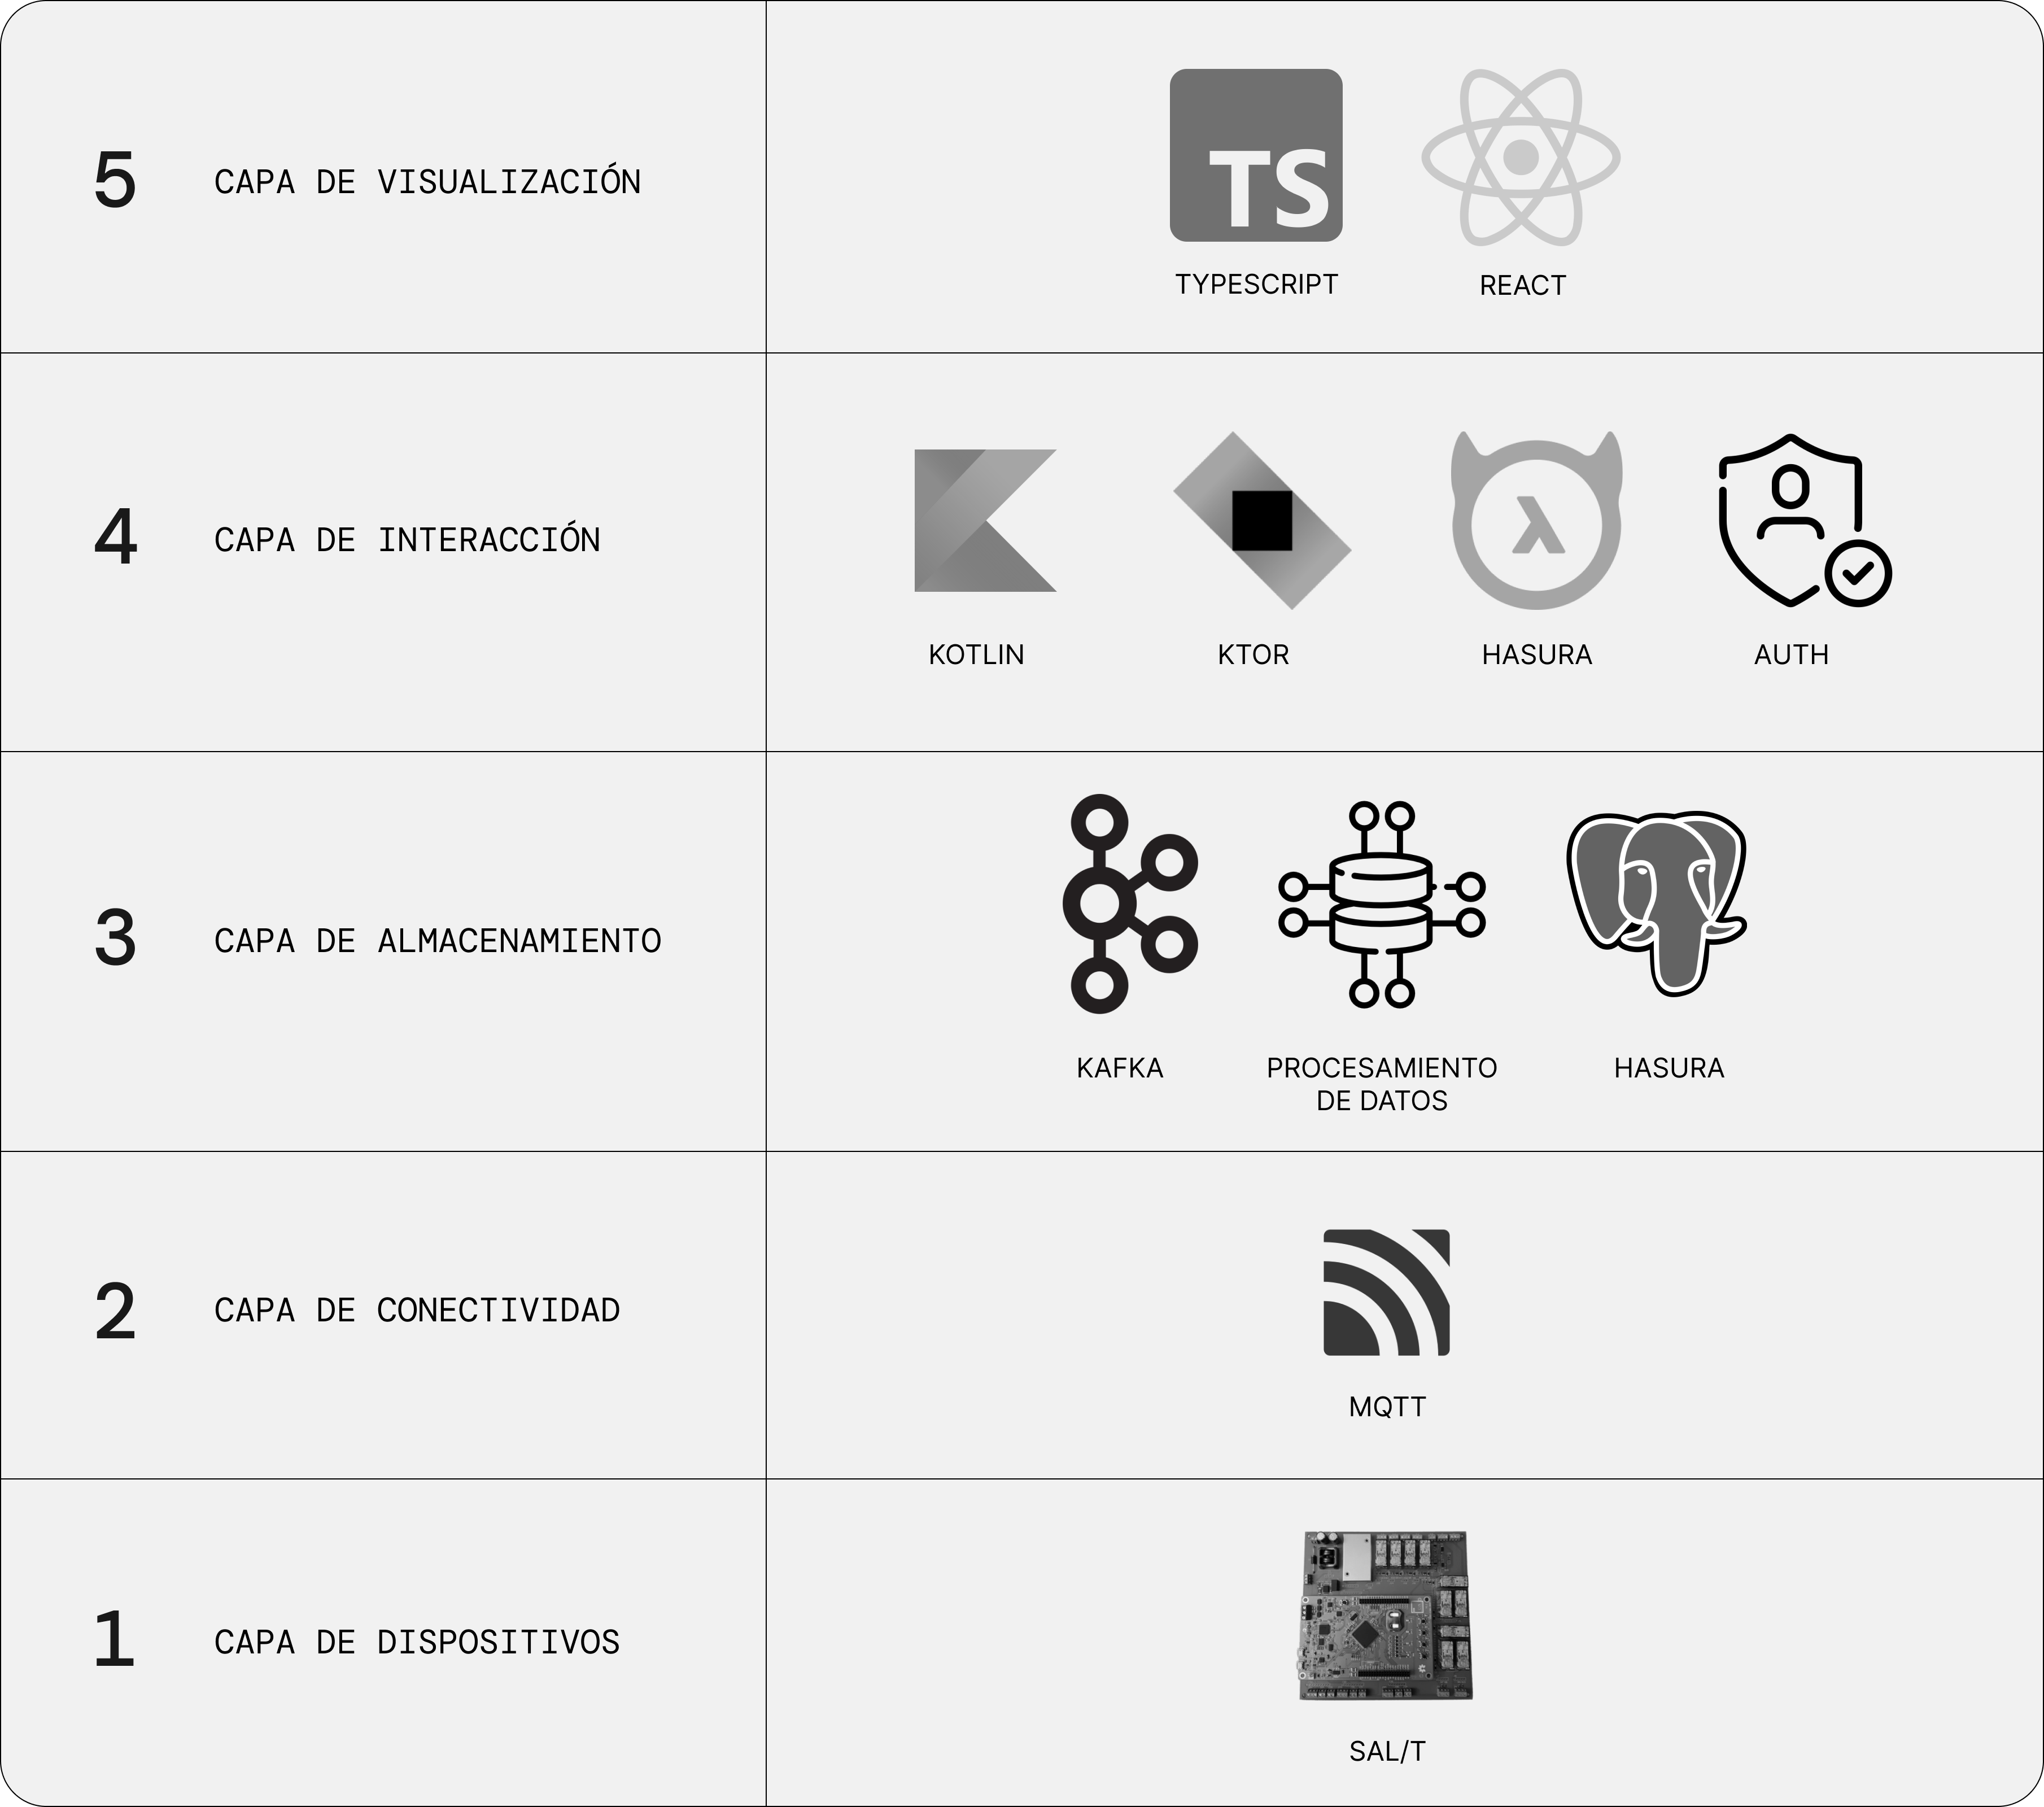
\includegraphics[width=.48\textwidth]{images/iot-stack-v2.1.png}
\caption{Arquitectura de la Central Operativa SAL/T.}
\label{fig:diagBloques}
\end{figure}


\subsection{Capa de dispositivos}

Sobre la base de un prototipo del Sistema de Aislamiento Limitado o Total, \textit{SAL/T}, se desarolló, en el kit de desarrollo \textit{Nucleo F429} \cite{b5}, un cliente \textit{MQTT} \cite{b6} que permite la publicación de la información proveniente de los subsistemas de falla, la velocidad de la información, entre otras variables; y llegado el caso, el dispositivo pueda realizar la lectura de diferentes parámetros configurables.

\subsection{Capa de conectividad}

Para la comunicación entre los dispositivos \textit{SAL/T} y la capa de almacenamiento, se utiliza un \textit{Broker MQTT} que oficia de orquestador entre el cliente, el dispositivo \textit{SAL/T}, que publica los mensajes y aquel que se suscribe, el sistema \textit{Kafka} \cite{b7}, para la lectura de la información y su posterior procesamiento. \\ 

Dado que los mensajes intercambiados entre las partes contienen información sensible, se ha optado por agregar la capa de seguridad \textit{TLS} \cite{b8}. En este sentido, resulta indispensable utilizar el certificado \textit{X509} \cite{b9} para prevenir ataques del tipo \textit{adversary-in-the-middle} \cite{b10} y utilizar certificados emitidos por autoridades reconocidas.


\subsection{Capa de almacenamiento}

La capa de almacenamiento por un lado se encuentra constituida por el sistema distribuido \textit{Kafka} que se encarga de almacenar los datos de la aplicación. Entre ellos se destacan los mensajes MQTT enviados por los dispositivos SAL/T, como también la información referida a las formaciones y a los SAL/T que las ocupan. \\

Además, se tienen servicios de procesamiento de datos que se encargan de adaptar la información de los tópicos en datos que posteriormente serán consumidos por los servicios que integran la capa superior. Por otro lado, se tiene una base de datos relacional \textit{PostgreSQL} \cite{b11} que se utiliza para almacenar los datos del servicio de autenticación y el motor que facilita la interacción con la plataforma web. Los conectores se encargan de insertar los datos que se quieran disponer a la capa de visualización.

\begin{figure}[ht]
\centering 
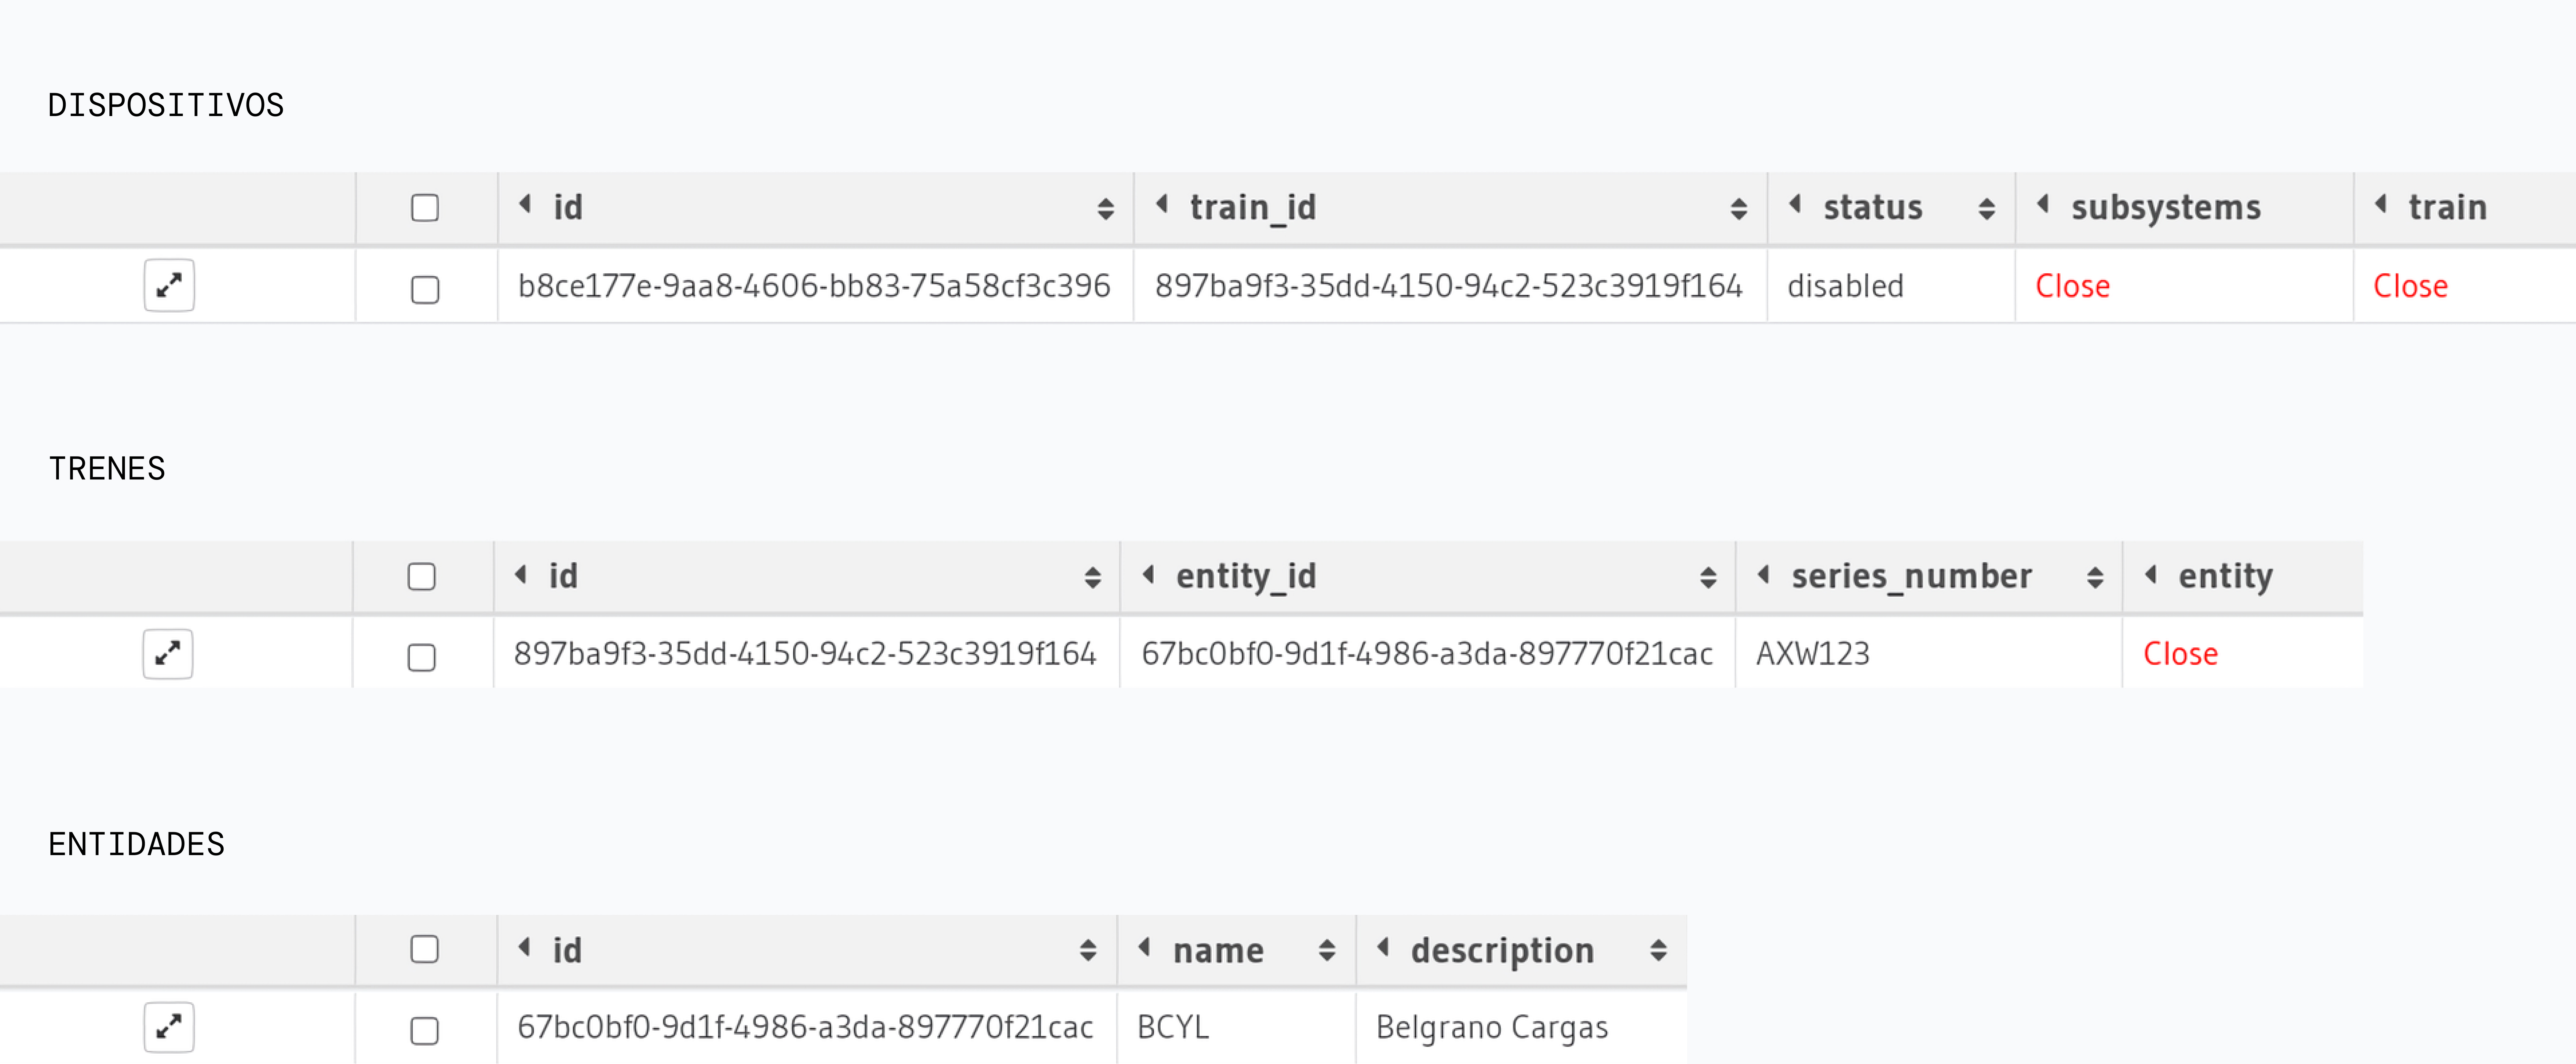
\includegraphics[width=.5\textwidth]{images/salt_table_v2.1.jpg}
\caption{Modelo de datos de los dispositivos, trenes y entidades.}
\label{fig:devicesTrainEntity}
\end{figure}

\begin{figure}[ht]
\centering 
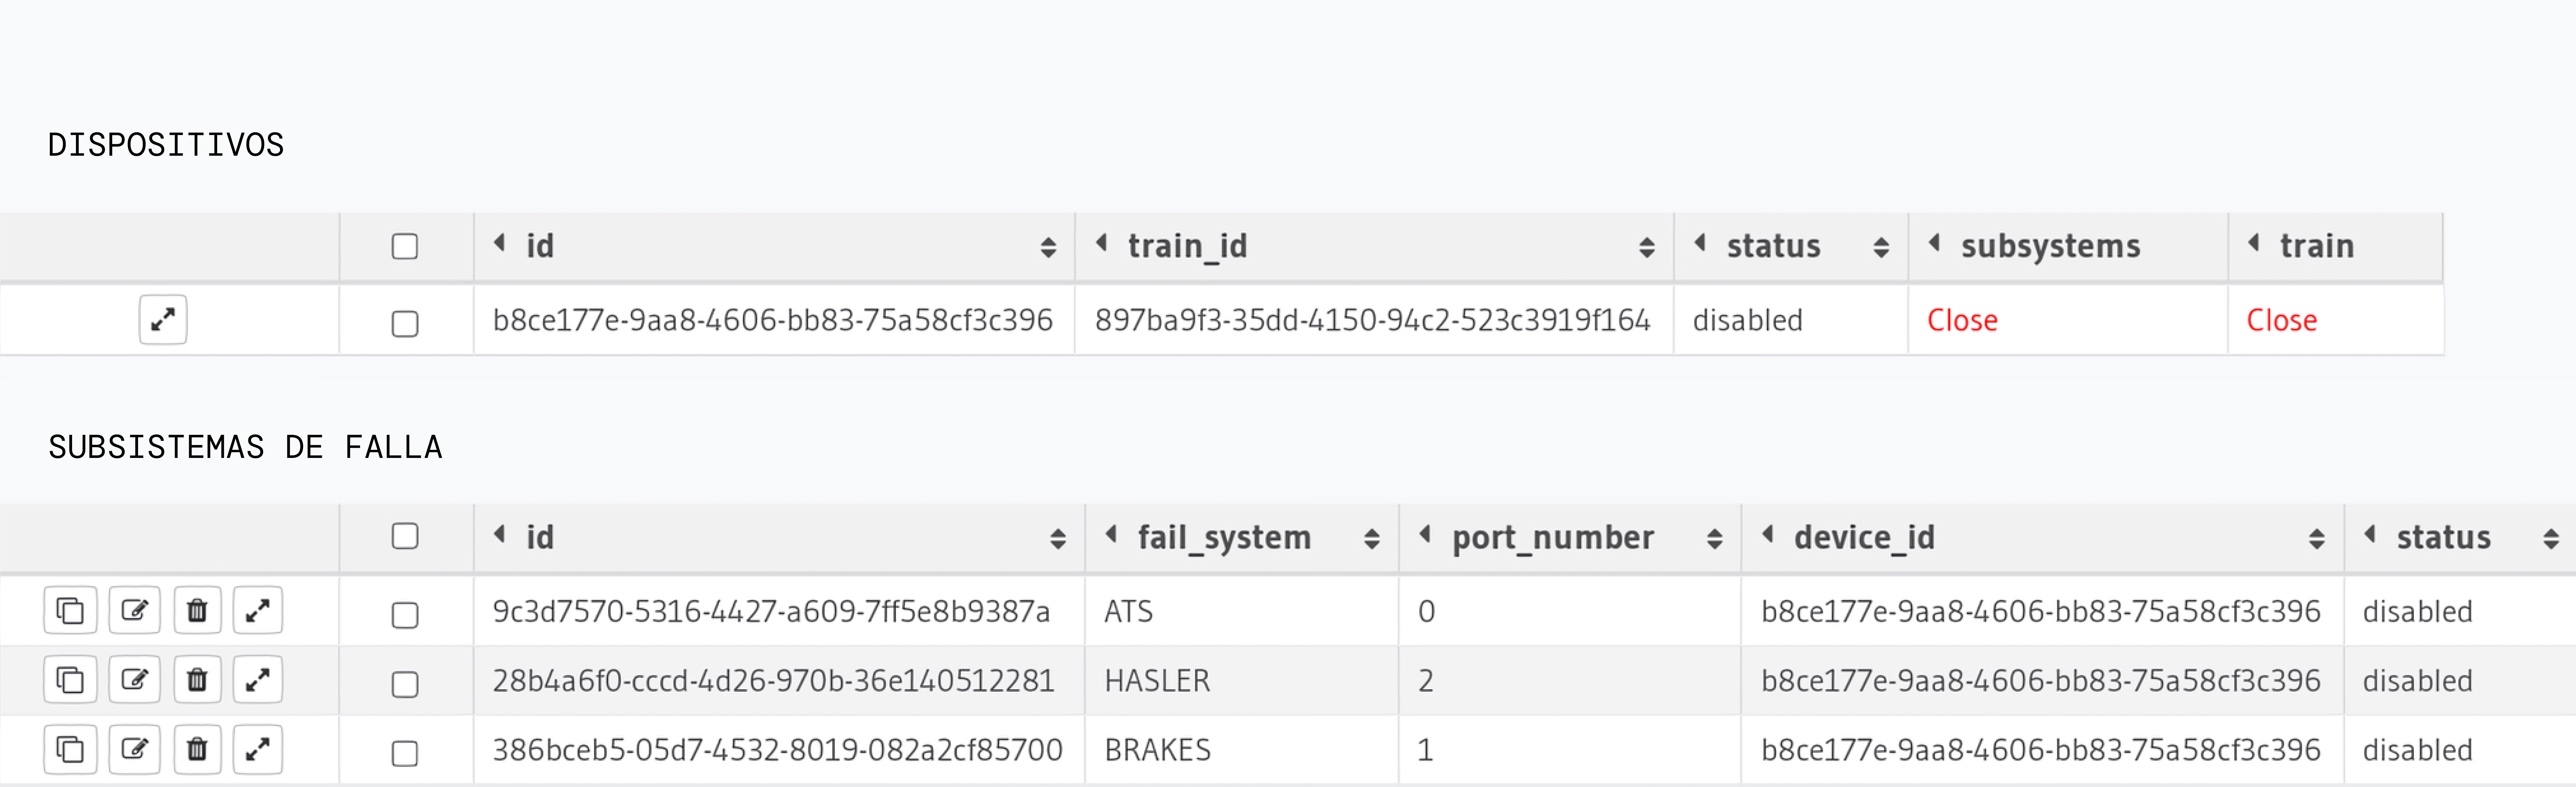
\includegraphics[width=.5\textwidth]{images/fail_system_v2.1.jpg}
\caption{Modelo de datos de los dispositivos y sus subsistemas de fallas.}
\label{fig:devicesSubsystems}
\end{figure}

En la figura \ref{fig:devicesTrainEntity} se observa el modelo de datos que representa a los dispositivos SAL/T, las formaciones y las entidades. 
El primero cuenta con un identificador del dispositivo en el sistema, el estado de operación y una referencia al tren en el que se desplegó el artefacto. 
El modelo de la formación está enriquecido con la entidad a la que pertenece y el numero de serie del tren. 
Por último, las entidades están compuestas por nombre y descripción.
Luego, en la imagen \ref{fig:devicesTrainEntity} se aprecian los subsistemas de fallas relacionados con el dispositivo SAL/T.
Su modelo esta integrado con el nombre del subsistema, el id del dispositivo al que está asociado y el estado actual del mismo. 

\subsection{Capa de interacción}

La capa de interacción se encuentra conformada por tres unidades. Por un lado, se ha desarrollado en el lenguaje \textit{Kotlin} \cite{b12} en conjunto con el \textit{framework} \textit{Ktor} \cite{b13} un microservicio de autenticación donde es posible la gestión de los usuarios con sus respectivos roles y también el \textit{backend}. Entre sus tareas principales se encuentran las relacionadas al protocolo \textit{MQTT} para la actualización de los certificados que brindan seguridad a las comunicaciones, mediante el uso de la capa de seguridad \textit{TLS}, y la indexación de los eventos que se publiquen en tiempo real; como la configuración general que permite el funcionamiento integral de los servicios y módulos dispuestos en el sistema. \\

Además, se dispone del motor \textit{Hasura} \cite{b14}, el cual se encuentra conectado a una base de datos relacional (\textit{PostgreSQL}) basado en el lenguaje de consulta estructurado \textit{SQL} \cite{b15} , que permite exponer una \textit{API GraphQL} \cite{b16} a aquellos clientes que deseen obtener una visualización del modelo de datos propuesto en que se conjuga la información de cada formación ferroviaria con su correspondiente dispositivo \textit{SAL/T} y diseño destinado al \textit{frontend}. Más aún, el enlace permite realizar modificaciones y hasta remociones de las columnas propuestas en las tablas de cada esquema dentro de la base de datos.


\subsection{Capa de visualización}

En esta capa, se ha utilizato el lenguaje de programación \textit{TypeScript} \cite{b17} junto con la biblioteca gráfica \textit{React} \cite{b18} para brindar una web reactiva en el que se elaboraron los formularios, las tablas y los paneles a partir de la explotación en de los datos almacenados en la base de datos. Cabe destacar que la plataforma web se encuentra condicionada por el rol y la entidad ferroviaria a la que pertenece cada usuario.

En la figura \ref{fig:dashboard} se puede apreciar el dashboard de la central operativa al que tendrán acceso los operadores de cada entidad.
En el mismo se observan distintas tarjetas con el estado de cada subsistema de fallas y del tren, como así también un velocímetro que
informa la velocidad de la formación.

\begin{figure}[ht]
\centering 
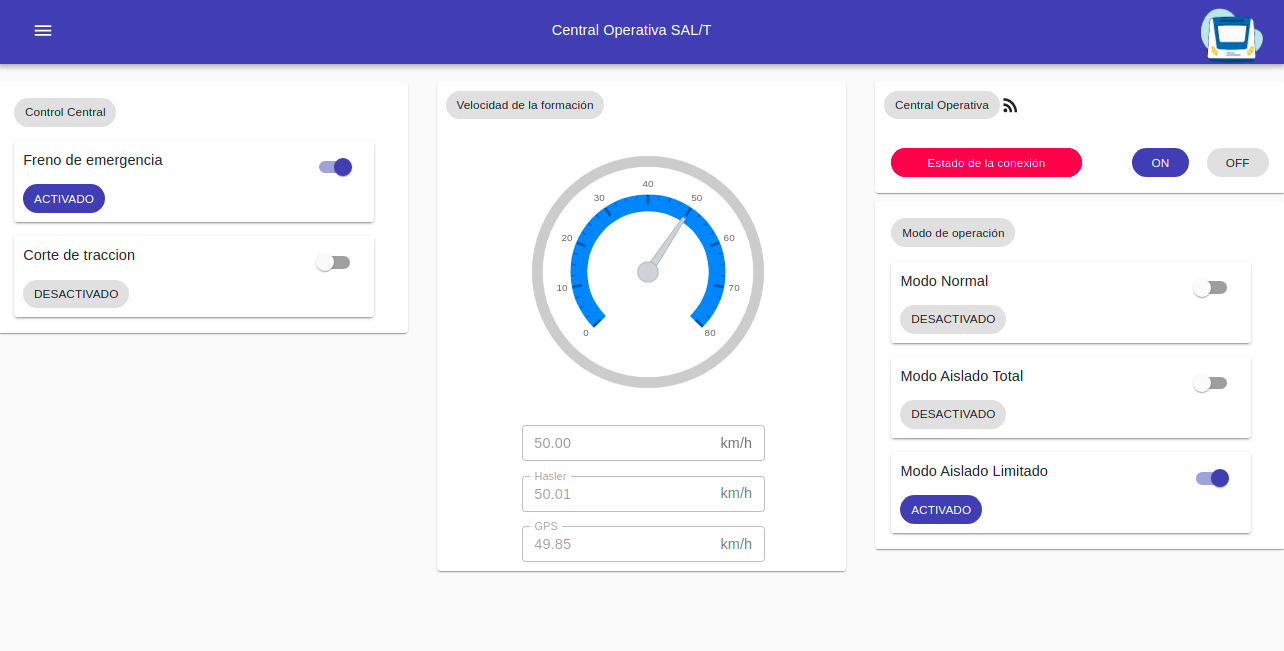
\includegraphics[width=.47\textwidth]{images/cental.png}
\caption{Panel de control de la central operativa.}
\label{fig:dashboard}
\end{figure}

\section{Conclusiones}

En este trabajo se presentan las principales características del diseño de una arquitectura en materia de \textit{software} y de \textit{firmware} para la operabilidad de los dispositivos SAL/T.
\\

Entre los módulos desarrollados, se posibilita la visualización de los usuarios y los dispositivos de cada entidad ofreciendo una solución sencilla y escalable. También, se cuenta la ingestión de la información recibida desde los dispositivos permitiendo una alta disponibilidad y operabilidad de los recursos. Por último, se cuenta con un microservicio destinado a la gestión de usuarios y perfiles que posee una alta tolerancia a fallos y adaptable.
\\

En la actualidad, se encuentra en desarrollo propiciar al operario enviar comandos de control a los dispositivos activos que tenga asignados, brindar la connfiguración de los parámetros de cada dispositivo y de ser deseable su correspondiente modificación y finalmente, brindar la seguridad en las comunicaciones agregando la capa \textit{TLS} en el protocolo \textit{MQTT}. 


\begin{thebibliography}{00}

\bibitem{b1} 'Sistema de supervisión de la seguridad del material
ferroviario utilizando patrones de diseño', Ivan Mariano Di Vito, Pablo Gomez, Ariel Lutenberg, Libro de trabajos del CASE2019, Congreso Argetino de Sistemas Embebidos, Santa Fe, Argentina. (2019).

\bibitem{b2} CONICET-GICSAFe (2022). [Online]. Disponible: \\
https://sites.google.com/view/conicet-gicsafe/inicio

\bibitem{b3} Trenes Argentinos (2022). [Online]. Disponible: \\
https://www.argentina.gob.ar/transporte/trenes 

\bibitem{b4} Introducción general a IoT (2022). [Online]. Disponible: \\
https://www.gotoiot.com/pages/articles/iot\_intro/index.html 

\bibitem{b5} NUCLEO-F429ZI (2022). [Online]. Disponible: \\
https://www.st.com/en/evaluation-tools/nucleo-f429zi.html

\bibitem{b6} MQTT (2022). [Online]. Disponible: https://mqtt.org/ 

\bibitem{b7} Kafka (2022). [Online]. Disponible: https://kafka.apache.org/  

\bibitem{b8} 'TLS/SSL - MQTT Security Fundamentals' (2022). [Online]. \\
Disponible: https://www.hivemq.com/blog/mqtt-security-fundamentals-tls-ssl/ 

\bibitem{b9} X509 (2022). [Online]. Disponible: \\
https://www.ssl.com/faqs/what-is-an-x-509-certificate/ 

\bibitem{b10} Adversary-in-the-Middle (2022). [Online]. Disponible: \\
https://attack.mitre.org/techniques/T1557/

\bibitem{b11} PostgreSQL (2022). [Online]. Disponible: https://www.postgresql.org/

\bibitem{b12} Kotlin (2022). [Online]. Disponible: https://kotlinlang.org/

\bibitem{b13} Ktor (2022). [Online]. Disponible: https://ktor.io/ 

\bibitem{b14} Hasura (2022). [Online]. Disponible: https://hasura.io/

\bibitem{b15} SQL (2022). [Online]. Disponible: https://www.w3schools.com/sql/

\bibitem{b16} API GraphQL (2022). [Online]. Disponible: https://graphql.org/

\bibitem{b17} TypeScript (2022). [Online]. Disponible: https://www.typescriptlang.org/

\bibitem{b18} React (2022). [Online]. Disponible: https://reactjs.org/


\end{thebibliography}

\end{document}












